\documentclass[10pt,a4paper]{article}
\usepackage{amsmath}
\usepackage{graphicx}
\usepackage[margin=1in]{geometry}

\catcode`\_=\active
\def_{\_}

\begin{document}

\begin{titlepage}
\title{G52GRP Interim Group Report\\HEX - A Chain Reactive Music Generator }
\author{Group NHN2}
\date{7th December 2012}
\maketitle
\thispagestyle{empty}
\begin{center}
Supervisor: Dr. Henrik Nilsson\\
\bigskip
\begin{tabular}{ l c r }
  S.Cooke & - & skc01u \\
  R. Fulton & - & rxf01u \\
  G. Hallam & - & goh01u \\
  D. Huo & - & dxh02u \\
  M. Tawafig & - & mxt41u \\
  J. Sherry & - & jxs41u \\  
\end{tabular}
\end{center}
\end{titlepage}

\tableofcontents
\pagebreak

\part{Preliminary Text}
\section{Concept}
\subsection{ReacTogon Concept}
The \textit{`ReacTogon`}\cite{modin} is a concept instrument produced by Mark Burton in 2007. Described as a `chain-reactive performance arpeggiator’, it acts as a physical user interface to a synthesiser through the placement of tokens on an interactive surface. The surface itself is a grid of hexagons, where each hexagon represents a musical note on the Harmonic table\cite{wikipediaHarmTab} - a novel method of placing musically complementary notes together, providing an easy and intuitive way to create chords and melodic sequences.\\

\begin{center}
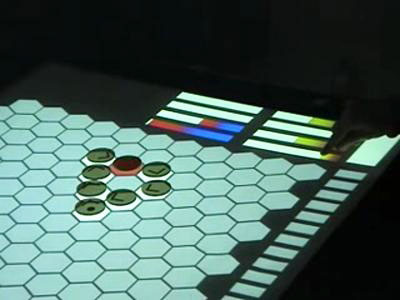
\includegraphics[scale=0.4]{1.jpg}\\
\textbf{The ReacTogon}
\end{center}

\subsection{Project Description}
Our project, branded \textit{`HEX’}, aims to emulate and extend the ReacTogon concept. Through the production of a software system that implements the harmonic table within the framework of a pattern based sequencer, we aim to provide a completely novel musical experience.\\
\\
To this end, we have written a Java applet that implements the harmonic table in this way. Control is provided through the use of five counters or `operator tiles’ that are placed onto the grid, namely Play, Stop, Change, Explode and Warp. The latter four have active and inactive states which dictate whether they play a note or not during an interaction. In addition to this there are buttons and sliders to change tempo and instrument. There are also multiple layers of grids, set out in tabs, for the creation of harmony and a multi textured composition.\\
\\
Our software is designed with a PC and touch screen in mind, as the tactile nature of interaction greatly lends itself to the interface. This said, the application will still run with a standard mouse and indeed, the nature of a Java applet allows portability and support for other operating systems.

\section{Background Information and Research}
\subsection{Existing Systems}
\subsubsection{Examples of Existing Software Systems}
\begin{enumerate}
\item \textbf{JR Hexatone Pro}
\begin{center}
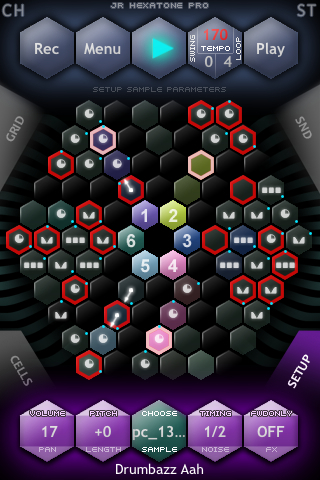
\includegraphics[scale=0.35]{2.jpg}
\end{center}
The JR Hexatone Pro is an application developed by Amidio for iOS that implements the harmonic table\cite{jrhexitunes}.  In a similar manner to the ReacTogon, tiles or `cell commands’ are placed on a circular grid of hexagons and control the nature of the sound produced. It’s unique selling point is derived from the fact that it uses `artificial intelligence and advanced randomisation algorithms’ to randomly alter the sound as the loop progresses to create a constantly changing sound. In addition to this, in place of a `start’ tile, sound is propagated from six `oscillator’ tiles at the centre of the grid and the playhead moves to one of three adjacent tiles. \cite{amidiomanual}

\item \textbf{TonePad / TonePad Pro}\\
The TonePad is another application for the iOS platform, developed by LoftLab.\cite{tonepaditunes} \\
\\
While it does not implement the harmonic table, it is based on a 16x16 matrix of notes in a pentatonic scale. To this end, it has a similar musical effect to notes played on a harmonic table. While the TonePad is simply controlled by selecting notes on the grid and has no placeable operation tiles, the ideas of playhead propagation and chain reactions are exemplified in this application. The playhead moves left to right across the grid and when a selected cell in the grid is encountered, it triggers others within a certain radius. \\
\\
A key feature of the TonePad application is it’s ability to import and export songs. Tracks can be exported as ringtones on iPhones or to m4r files. It is also possible to export song ‘code’ for sharing with others; this is integrated into the app with an ‘upload’ button. 
\end{enumerate}

\subsubsection{Examples of Existing Hardware Systems}
\begin{enumerate}
\item Tenori-On
\begin{center}
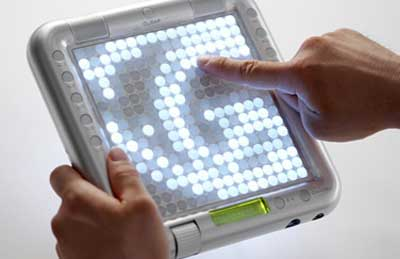
\includegraphics[scale=0.5]{3.jpg}\
\end{center}
Developed in 2005 by Japanese artist Toshio Iwai and Yu Nishibori at Yamaha\cite{tenorionwiki}, the Tenori-On is a hand-held music sequencer. Fundamentally, it is conceptually similar to the TonePad, but in hardware form and with a variety of different modes. The hardware itself consists of a 16 x 16 matrix of pressable buttons which light when activated. These buttons can act in a similar manner to the cells in the TonePad in the main sequencing mode, where highlighted cells are played when the playhead encounters them.\\
\\
In addition to this, five other modes exist such as `push mode’, which produces a continuous sound when a cell is pressed; `bounce mode’ which causes a the playhead to oscillate between the selected cell and the edge of the matrix, producing sound when `bouncing’ off the side and `grouping’ which is used to sequence patterns together.\\
\\
Each loop is composed within a layer and each layer can be thought of as `performance parts' of which there can be a total of sixteen. Different notes and instruments can be assigned to each layer and all layers can be played together in synchronisation. Each set of sixteen layers is called a block; a total of sixteen blocks can be stored and dynamically switched between in performance. In this way, musical loops and motifs can be generated and played sequentially to create a complete piece of music\cite{tenorionyamaha}.

\item \textbf{AXiS-64}
The AXiS-64 is possibly the most prevalent MIDI controller and piece of hardware that utilises the harmonic table. The equipment itself consists of the keyboard itself, composed of 192 hexagonal keys; 8 preset keys for storage of user defined keyboard configurations; 4 cursor keys, for navigating between banks; a pitch bend wheel; a modulation wheel and two rotary dials\cite{cthru}. The four analogue interfaces can be easily reprogrammed and used for any MIDI controller change.
\begin{center}
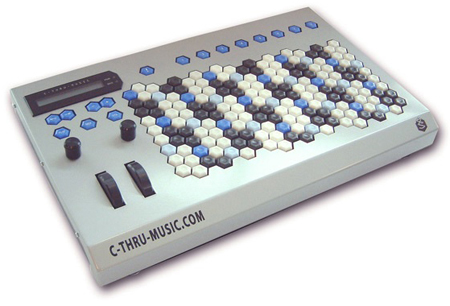
\includegraphics[scale=0.5]{4.jpg}
\end{center}
The fourth revision of the AXiS-64 firmware introduced three different keyboard modes; `single’, `split’ and `layer’.  In ‘split’ mode the keyboard is split into three 64 note keyboards; in layer it becomes one keyboard sending a signal on up to three MIDI channels when a note is played and in `single’ it acts as a single keyboard.
\end{enumerate}
\subsection{Systems Research Evaluation}
The products listed above are but a few among the systems available on the market, but each one exhibits interesting or unique characteristics that can be taken as inspiration for our project. In addition to this, there are persistent themes among all products that too will influence our designs.\\
\\
Among these common themes is the use of physical interaction as an interface between the system and the user. A considerable majority of the software systems available are for tablets or mobile devices using touch screen interfaces, with almost no standard desktop applications and only a few online hardware simulations or alternatives. This information justifies our choice of using a touch screen interface with our software.\\
\\
In addition to this, particularly interesting features of researched products that we may wish to take forward into our project include the multiple `layers' featured in the Tenori-On and the TonePad Pro's ability to export and share music and created projects. 

\subsection{Market Research}
TO BE COMPLETED
\subsection{Music Research}
\begin{center}
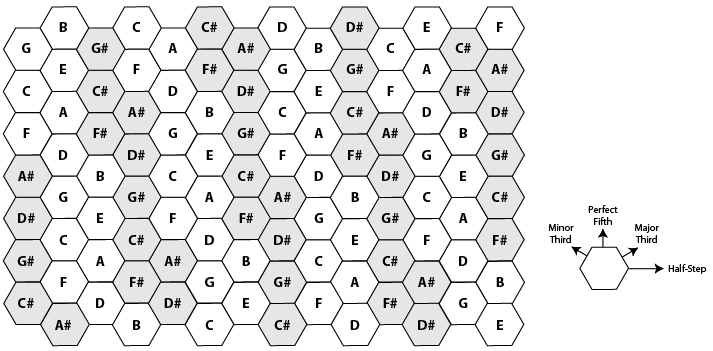
\includegraphics[scale=0.5]{5.png}
\end{center}
In musical theory, an interval is the distance between two notes or pitches. Typically, these are represented with tones and semitones, where tones are the base unit of an interval. Certain intervals appear particularly often within music and composition as they can provide key melodies. Such intervals include the perfect fifth, and major and minor thirds. These intervals, which are 7, 4 and 3 semitones above the base note respectively, make up the notes used in major and minor triads and are the intervals used in the harmonic table based on the following set of rules:\\
\\
\begin{itemize}
\item Notes ascend by an interval of a fifth on the vertical axis.
\item Notes ascend by an interval of a major third on one diagonal axis.
\item Notes ascend by an interval of a minor third on the other diagonal axis.
\end{itemize}
This layout clusters complementary notes together, for example, all the notes in the C Major chord, namely C, E and G are adjoining. Scales are played by using simple, repeated patterns that can be transposed for playing in different keys. In this way, music can be easily and quickly created.\\
\begin{center}
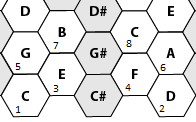
\includegraphics[scale=0.7]{scale.png}
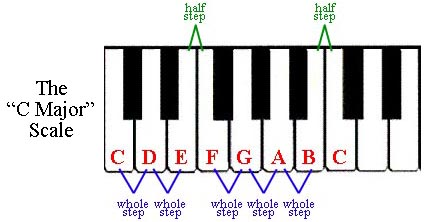
\includegraphics[scale=1.5]{scale2.jpg}
\end{center}
Above is shown a comparison of the C major scale played on a harmonic table based keyboard (left) and on a conventional piano keyboard (right). The progression is enumerated from 1 to 8.\\
\\
Scales and triads can be transposed far more easily on a harmonic keyboard than on a conventional keyboard as the basic pattern is always retained. This is shown in the G major scale below:
\begin{center}
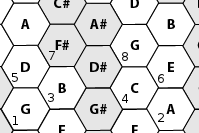
\includegraphics[scale=0.5]{scale3.png}
\end{center}
\subsection{Technical Research}
\subsubsection{MIDI}

\subsubsection{Working with Hexagons}

\section{Requirements Specification}
Our project has several important key features which need to be followed and implemented; they can be described in the functional, in other words, definitions of what the system must do; and non-functional requirements, definitions of how the system is supposed to be. These are detailed henceforth:
\subsection{Functional Requirements}
\begin{enumerate}

\item The application must be able to play a note at the press of a hexagonal tile on the grid.
\begin{enumerate}
\item It must be possible to manipulate the sound through variation of voice/MIDI instrument.
\end{enumerate}

\item The application must implement the Harmonic Table in the layout of playable notes.
\begin{enumerate}
\item The notes must be set out on a grid of contiguous hexagons.
\item Moving immediately up a hexagon will increase the pitch by an interval of a 5th and vice versa.
\item Moving immediately right a hexagon will increase the pitch by a semitone and vice versa.
\end{enumerate}

\item `Operator tiles' should be placed on individual hexagons within the grid to manipulate sound in various ways.

\item The following operator tiles should be implemented:
\begin{enumerate}
\item \textit{Play} - Begins the sequencer, sending an initial pulse in a straight line in a specified direction.
\item \textit{Stop} - Stops and `absorbs' the pulse at that position.
\item \textit{Change} - Changes the direction of the pulse.
\item \textit{Explode} - Causes the pulse to `split’, propagating new playheads from each edge of the hexagon it is placed on, but not going back on itself.
\item \textit{Warp} - When the playhead meets a warp tile, it will spawn new playheads at each other warp tile placed on the grid, moving in the direction of entry. 
\end{enumerate}

\item Tempo must be controlled in two ways:
\begin{enumerate}
\item A global base tempo must be set.
\item Tempos on each grid can be set independently.
\begin{enumerate}
\item Individual grid tempos must be a multiple of two, relative to one another.
\end{enumerate}
\end{enumerate}

\item A moving `pulse' or `playhead' should be used to trigger tiles placed on hexagons.
\begin{enumerate}
\item The playhead must move faster or slower based on the tempo specified.
\item The playhead must move consistently with the tempo specified.
\end{enumerate}

\item Each operator tile should have an off or an on status, which dictates whether it will play a note when encountered by a pulse.
\begin{enumerate}
\item The sound produced is based on the position of the tile on the harmonic table grid, rather than the tile itself.
\end{enumerate}

\item Operator tiles should be removed with a delete mechanism.
\begin{enumerate}
\item When a `delete' key is depressed, a click must remove a tile from the grid.
\item There must be a `clear' button to remove all tiles from an individual grid.
\end{enumerate}

\item The following operator tiles must be able to rotate when placed in order to send the playhead in different directions:
\begin{enumerate}
\item \textit{Play}
\item \textit{Change}
\end{enumerate}

\item Six grids should be implemented for use in harmonic, polyphonic projects.
\begin{enumerate}
\item Grids must be independent.
\item Different tiles must be able to be placed on different grids.
\item Each grid must be able to have it's own tempo.
\item Grids must be able to be played simultaneously.
\end{enumerate}

\item Global `Start' and `Stop' buttons should be implemented to start and stio playheads over all grids.
\begin{enumerate}
\item Individual grids must be able to be selected and deselected for play.
\end{enumerate}

\item Saving and loading must be implemented for ease of producing and sharing projects.
\begin{enumerate}
\item Individual grids must be able to be saved independently
\item Projects must be able to be saved as a whole.
\end{enumerate}

\item The application must implement a control system suitable for a touch screen and also mouse interface.
\begin{enumerate}
\item The application must be controlled through use of single touch sliders and buttons.
\item It must have either `tap to scroll' and/or `drag and drop' selection.
\item Menus must be available through a single click mechanism.
\end{enumerate}

\item The menu must contain at least the following key features:
\begin{enumerate}
\item Create new project.
\item Save/Load.
\item Select Grid.
\item Change instrument on a certain grid.
\item Select grids to play.
\item Open help screen.
\end{enumerate}


\end{enumerate}
\subsection{Non-Functional Requirements}
Our application is aimed to be used by a wide variety of people, with varying levels of musical capability. With this in mind we must place much effort into making the application as accessible and easy to use as possible. As such, it is important that our project conforms to the following principles:

\begin{enumerate}
\item Extensibility - The application should be fully extensible, i.e. adding new features, and carry-forward of upgrades should be viable while maintaining the core mechanic.
\item Maintainability - The application should be easy to maintain.
\item Performance - The application should run comfortably on a wide range of computers.
\item Usability - the application should be easy to use and have simple, intuitive user input.
\end{enumerate}

\part{Design}
\section{Software Design}
We looked at the Reactogon and decided to expand upon it, please look at the functional requirements for this.
\subsection{The Grids}
OUr software would comprise of 6 layers; each layer being a grid. Each grid would have to be unique yet have different properties; this was the first clue to using OO design. Each grid would have a set of properties, these properties being:
\begin{itemize}
\item Each grid could be assigned a unique instrument, but needs to support changing it on the go during mid play. This suggested that a grid could be assigned its own channel in a MIDI sequencer. (Rees, 2001)

\item Each grid could support different octaves, through the research we found that MIDI can play 127 different notes ranging from octaves 0 to 10, our grids therefore need to be able to be transposed mid session. This suggests that each grid have a starting note and some sort of algorithm then fills the grids with correct notes.\\
\\
The tempo of the grid should be changeable, but all grids needs to have some sort of relation to each other, so some sort of base tempo needs to be applied, then each grid can then play at $ 1 \times , \frac{1}{2}, \frac{1}{4}, \frac{1}{8}$ or $\frac{1}{16} $ times that pace, these values were chosen due to the research in music theory. This implies that a grid can be halted for set amount of time/tick.
\end{itemize}

The grid itself would be made up of hexagonal `cells’, these should hold information about what note each cell is, this could simply be a number. From this it would be sensible to store the cells as a 2D array. As discussed above this would then make it quite simple to transpose notes with an algorithm. Information about where it should be placed in the grid itself. Some of the properties of hexagons are outlined in the research and will help for placement and using hexagon properties to our advantage. Because this is quite a visual piece of software some information needs to be held about its state, as we wanted to show if a cell is active or not.

\subsection{Pulse}
The vision of a pulse is some sort of object moving through the grid, from cell to cell. The pulse itself should be quite simple as all it must do is move from one cell to another. The tempo of the grid should manipulate how fast the pulse moves from one to another. The grid must be able to support multiple pulses, all moving in different directions at the same time. As well as this, pulses must not affect one and other, crossing/colliding pulses shouldn't be a problem and the software must be able to handle this. But the software must be able to handle pulses that occupy the same space, as not to create exponential loops see figure 1. When a pulse comes into contact with a tile it should affect the pulse in some way.
\begin{center}
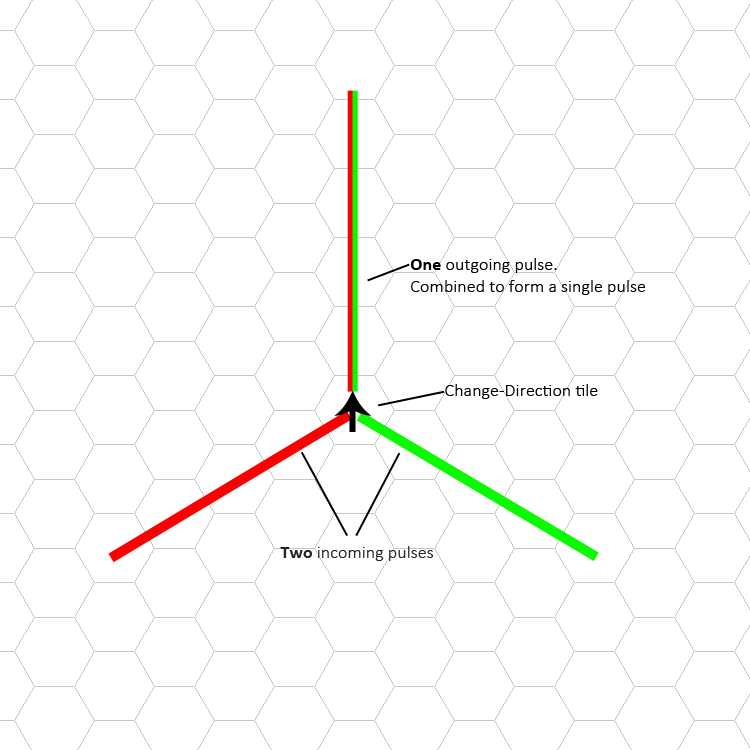
\includegraphics[scale=0.5]{6.png}
\textbf{fig. 1}
\end{center}

\subsection{Tiles}
The main idea of this software is the use of tiles to manipulate the music. A tile can be placed in a cell on the grid and used to manipulate an incoming pulse. Different tiles have different effect. The tiles are listed as follows:
\begin{itemize}
\item    Stop: Should destroy the pulse

\item Change direction: This implies that the tile should hold a direction and then be able to pass this information onto an incoming pulse. Because the tile will have different arrows for different locations will mean that the graphics will have to be redrawn with the corresponding arrow.

\item Play: Will work in much the same way as change direction as it should be able to change a pulses direction. As well as this it will be the starting position of a pulse, maybe creating it.

\item Explode: Will destroy and incoming pulse in much the same way as stop does, but in turn create 5 new ones and send them in every direction apart from the input. From this knowledge it would be sensible to assume that a pulse should hold information about its previous position in the grid.

\item Warp: Will ‘warp’ a pulse from one place to another,  if multiple warps are places then the pulse should come out of those tiles also. From this I will make a warp tile destroy a pulse, and create new ones in all output locations. There will need to be some way of storing locations of all warp tiles in a grid, all with their own unique id.
\end{itemize}

The tile object should therefore have a ‘type’ and a direction at minimum. When I pulse comes in contact with a tile it should play a note, but there are also tiles that should not play a note, this means there must be some data variables stored in each time if it should play a note or not when hit by a pulse.

\subsection{Keeping Time}
The whole system needs to be produce music at a reliable rhythm, therefore there needs to be some timer that tells each grid to increment all the pulses why one step. The timer must always have the same interval.

\subsection{Creation of Sound}
If 4 separate pulses hit 4 different tiles on the same ‘tick’, they all should be played at the exactly the same time, and all 6 grids must follow this rule. For this to happen, there needs to be some sort of queue, where all notes that should be played at a set point in time are grouped together, then sent off to be played all at once. This could happen multiple times per second, so it looks like some sort of thread will be needed to play multiple sequences at the same time and will not halt the program.

\section{User Interface Designs}
TO BE COMPLETED


\part{Implementation}
\section{Key Control Elements}
\subsection{Removal of Duplicates}
Removal of duplicates, figure 1 in the design shows a problem of pulses merging together. Two or more pulses could occupy the same space and this would cause the amount of pulses to exponentially grow and in turn cause the program to slow down and eventually crash.\\
\\
This was due to pulses being held in an array, to removing duplicates from this array would take $ O(n^{2}) $ time, and even then it would still have problems detecting them. To solve this problem, a hash map was used to store the location of the pulse in the grid. The hashing algorithm took the pulses current location, and direction to place it in the hash map, the hashing algorithm is shown in below (equation 1). The hashing algorithm was relatively simple because by virtue of using hexagons it was possible to work in base 6. By doing this, if two pulses occupied the same space on the gird (going the same direction etc.) they would be placed in the same position in the hash table; this would cause a collision, but as a hash table only accepts unique values, the second value (and any after that) would simply write over the old value. See the Hash Maps section of Technical Research for more.\\
\\
To keep track of the keys in the hash map there is an array list holding all the keys that are currently in use, to access the pulses it was necessary to traverse through this list and use the keys to get data from the hash map. Every loop, the array list was emptied and all keys where added again. By using a hash map access time was reduced to $O(1)$ and removal was never a problem, as a hash map with no linear probing just writes over a value. It also meant I was not adding and removing lots of pulses from an array list all the time.\\
\begin{equation}
Key = ((Pulse.tLocation \times 36) + (Pulse.fLocation \times 6) + direction)
\end{equation}

\subsection{Timing and Tempo}
Timing the whole system was very important. To do this I used Timer that was scheduled at a fixed rate. This meant that it would call the run method every set amount of time irrespectively if it had finished the methods or not. See figure 2. The timer controlled how often the pulses moved one space in the grid. Because each grid could have a different tempo I needed to keep all the grids synchronised but still have different tempos. To do this in grid a tempo is assigned with a value of 1, 2, 4, 8, or 16.\\
\\
Then every loop of the base timer a value is incremented by 1 this value is then MODed against the tempo of each grid, if it is 0 then it will move the pulses inside this grid by one, it if it not it will skip this grid. This is explained clearly in the below code for the \textit{play()} method. At the end of every loop queues of notes are played, this keeps everything in sync.\\
\begin{center}
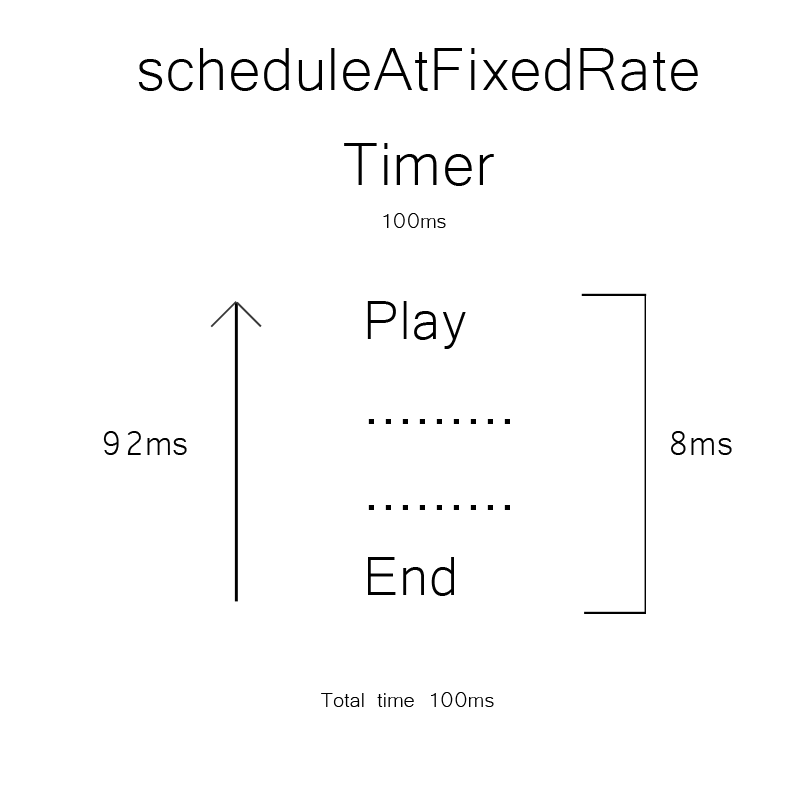
\includegraphics[scale=0.2]{utimer.png}
\end{center}
\subsubsection{\textit{play()} method Implementation}
\begin{center}
\begin{verbatim}

function play() 
    if (tempoControl > 16) 
        tempoControl = 1 
    for all grids 
        if (tempoControl % grid.getTempo == 0) 
            grid.play() 
    tempoControl++
    playNotes() 
	
\end{verbatim}
\end{center}

\subsection{Transposition}
\begin{center}
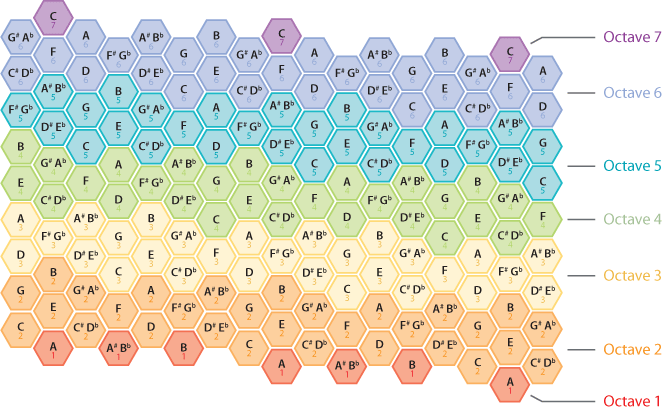
\includegraphics[scale=0.5]{7.png}
\end{center}
One feature of the program that was much easier to implement than expected was being able to transpose the whole grid and changing the start note of each grid on the fly. You could use the fact hexagons where stored in a 2nd to your advantage and that MIDI notes could be stored as numbers. Studying how the harmonic table works (figure 5), and finding patterns how the notes were placed we were able to write a simple formula (figure 6), that selecting a start node of the grid, it could then place the correct notes in the correct place. Putting this formula then in a loop that goes through the array meant it could be called at any time even during play, as hexagon cells themselves held the note numbers. This formula would work for any size grid, so if we wanted to extend the table at some point that would be possible. 

\section{Implementation of Data Structures and Methods}
\subsection{Timers}
\subsection{Hexagon Cells}
\subsection{Images}

\section{Testing}
sdtujstyuj

\part{Project Meta-Comment}
hdghsghh
\section{Updates since Interim Report}

\section{Time and Planning}

\section{Problems Encountered}


\part{Conclusion}

\part{Appendices}
klujghf;kjghglkjghslkjh
\section{References}
\bibliographystyle{IEEEtran}
\bibliography{reportReferences}

\end{document}